\documentclass[tikz,convert={outfile=\jobname.svg}]{standalone}
%\usetikzlibrary{...}% tikz package already loaded by 'tikz' option
\begin{document}

\newcommand*{\xMin}{-6}%
\newcommand*{\xMax}{8}%
\newcommand*{\yMin}{-5}%
\newcommand*{\yMax}{6}%


\newcommand{\epuck}[3][0] % [angle]{x}{y} avec angle optionel
{
	\draw [very thick, fill=white] (#2,#3) circle [radius=0.5];
	\draw [very thick, rotate around={#1:(#2,#3)}] (#2-0.25,#3-0.433) -- (#2,#3+0.45) -- (#2+0.25,#3-0.433);
}

\newcommand{\epuckred}[3][0] % [angle]{x}{y} avec angle optionel
{
	\draw [very thick, fill=white] (#2,#3) circle [radius=0.5];
	\draw [red, very thick, rotate around={#1:(#2,#3)}] (#2-0.25,#3-0.433) -- (#2,#3+0.45) -- (#2+0.25,#3-0.433);
}

\newcommand{\human}[3][0] % [angle]{x}{y}
{
	\draw [fill=white, line width=1.5pt, rotate around={#1:(#2,#3)}] (#2,#3+1) -- (#2-0.866,#3-0.5) -- (#2+0.866,#3-0.5) -- cycle;
	\draw (#2,#3) node[scale=2, rotate around={#1:(#2,#3)}]{H};
}
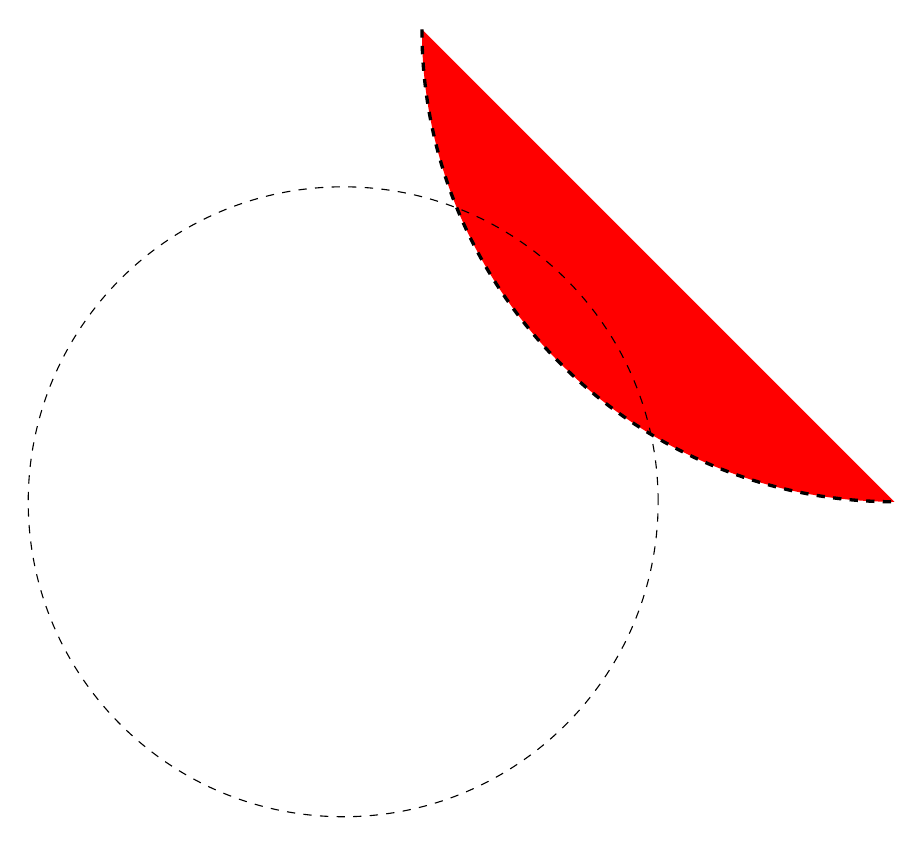
\begin{tikzpicture}

%	\foreach \i in {\xMin,...,\xMax} {
%        \draw [very thin,gray] (\i,\yMin) -- (\i,\yMax)  node [below] at (\i,\yMin) {$\i$};
%    }
%    \foreach \i in {\yMin,...,\yMax} {
%        \draw [very thin,gray] (\xMin,\i) -- (\xMax,\i) node [left] at (\xMin,\i) {$\i$};
%    }
	
	\draw [very thick, dashed, fill=red] (2,6) arc [radius=6, start angle=180, end angle=270];
	
	\human{1}{0}
	
	\draw [dashed] (1,0) circle [radius=4];
	
	\epuckred{2.5}{3.5}
	\epuckred{3.5}{2}
	\epuckred{4.9}{0.8}
	\epuck{4.9}{-1}
	\epuck{4}{-2.5}
	\epuck{2.5}{-3.6}
	\epuck{-2.9}{-1}
	\epuck{-2}{-2.5}
	\epuck{-0.5}{-3.6}
	\epuck{-2.9}{1}
	\epuck{-2}{2.5}
	\epuck{-0.5}{3.6}

\end{tikzpicture}
\end{document}